% Wind-load induced segment piston of the GMT, for an adaptive optics audience
% Build with: latexmk -xelatex windloads-segement-piston.tex
% Figures: python3 make_figures.py <data> <fem> (see make_figures.py)
\documentclass[10pt,aspectratio=169]{beamer}
\usetheme[progressbar=frametitle,numbering=fraction,sectionpage=none]{metropolis}
\usepackage{booktabs}
\usepackage{siunitx}
\usepackage{tikz}
\usetikzlibrary{arrows.meta,positioning,fit,calc}
\sisetup{group-separator={,},group-minimum-digits=4}

\definecolor{ink}{HTML}{23373B}
\definecolor{accent}{HTML}{2A78D6}
\definecolor{warm}{HTML}{E2622A}
\definecolor{soft}{HTML}{EEF1F5}
\definecolor{softblue}{HTML}{DCE9FA}
\definecolor{softwarm}{HTML}{FCE5D9}
\setbeamercolor{alerted text}{fg=warm}
\setbeamercolor{frametitle}{bg=ink}
\setbeamercolor{progress bar}{fg=accent,bg=soft}

\tikzset{
  box/.style={draw=none,fill=#1,rounded corners=3pt,align=center,inner sep=5pt,font=\small,minimum height=1.1cm},
  box/.default=soft,
  flow/.style={-{Stealth[length=2.2mm]},thick,draw=ink!70},
}

\title{Wind-load induced segment piston of the GMT}
\subtitle{From CFD wind loads to segment piston, through the integrated model}
\author{R.\,Conan}
\institute{GMTO integrated modeling}
\date{November 2026}

\begin{document}

\maketitle

%------------------------------------------------------------------------------
\begin{frame}{Why segment piston from the wind matters}
  \begin{columns}[T]
    \begin{column}{0.55\textwidth}
      \small
      \begin{itemize}
        \item Wind buffets the telescope structure inside the enclosure: the 7 M1 and 7 M2 segments move as rigid bodies
        \item The resulting \alert{segment piston} is a differential path length between the 7 sub-apertures of the GMT pupil
        \item Piston is invisible to slope-based wavefront sensors: it must be measured and corrected by the phasing sensors and the M2 piston control
        \item Its amplitude and temporal spectrum set requirements on these loops
      \end{itemize}
    \end{column}
    \begin{column}{0.4\textwidth}
      \begin{block}{This talk}
        \begin{enumerate}
          \item The models and the data pipeline
          \item Sensitivity to the structural damping
          \item Segment piston over the 63 CFD wind cases
        \end{enumerate}
      \end{block}
      \vspace{2mm}
      {\small All piston values are \alert{wavefront} piston in the exit pupil, in nm; std is over \SI{395}{s} at \SI{1}{kHz}.}
    \end{column}
  \end{columns}
\end{frame}

%------------------------------------------------------------------------------
\section{Models and data pipeline}

\begin{frame}{The integrated model at a glance}
  \centering
  \resizebox{0.97\linewidth}{!}{%
  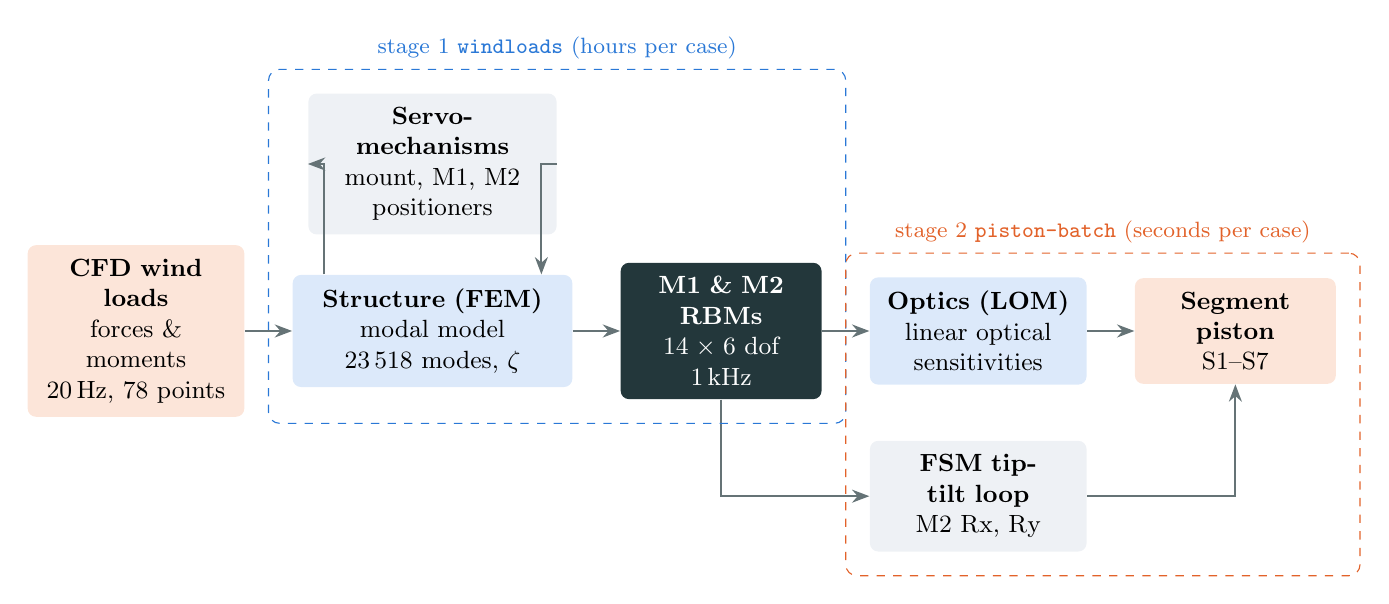
\begin{tikzpicture}[node distance=7mm and 6mm]
    \node[box=softwarm,text width=2.4cm] (cfd) {\textbf{CFD wind loads}\\forces \& moments\\\SI{20}{Hz}, 78 points};
    \node[box=softblue,text width=3.2cm,right=of cfd] (fem) {\textbf{Structure (FEM)}\\modal model\\\num{23518} modes, $\zeta$};
    \node[box,text width=2.8cm,above=5mm of fem] (ctrl) {\textbf{Servo-mechanisms}\\mount, M1, M2\\positioners};
    \node[box=ink,text=white,text width=2.2cm,right=of fem] (rbm) {\textbf{M1 \& M2 RBMs}\\$14\times6$ dof\\\SI{1}{kHz}};
    \node[box=softblue,text width=2.4cm,right=of rbm] (lom) {\textbf{Optics (LOM)}\\linear optical\\sensitivities};
    \node[box=softwarm,text width=2.2cm,right=of lom] (out) {\textbf{Segment piston}\\S1--S7};
    \node[box,text width=2.4cm,below=7mm of lom] (fsm) {\textbf{FSM tip-tilt loop}\\M2 Rx, Ry};
    \draw[flow] (cfd) -- (fem);
    \draw[flow] (fem.north west) ++(4mm,0) |- (ctrl.west);
    \draw[flow] (ctrl.east) -| ($(fem.north east)+(-4mm,0)$);
    \draw[flow] (fem) -- (rbm);
    \draw[flow] (rbm) -- (lom);
    \draw[flow] (lom) -- (out);
    \draw[flow] (rbm.south) |- (fsm.west);
    \draw[flow] (fsm.east) -| (out.south);
    \node[draw=accent,dashed,rounded corners,fit=(fem)(ctrl)(rbm),inner sep=3mm,
      label={[accent,font=\footnotesize]above:stage 1 \texttt{windloads} (hours per case)}] {};
    \node[draw=warm,dashed,rounded corners,fit=(lom)(out)(fsm),inner sep=3mm,
      label={[warm,font=\footnotesize]above:stage 2 \texttt{piston-batch} (seconds per case)}] {};
  \end{tikzpicture}}
  \vspace{3mm}

  {\small The time domain simulation runs at \SI{1}{kHz}: the CFD loads drive the structure, which is held in place by its own control loops; the optics are a linear function of the rigid body motions (RBMs).}
\end{frame}

%------------------------------------------------------------------------------
\begin{frame}{Wind loads: 63 CFD cases}
  \begin{columns}[c]
    \begin{column}{0.39\textwidth}
      \begin{itemize}
        \item Transient CFD of the telescope in its enclosure (2025 campaign)
        \item Forces and moments on 78 structural surfaces: M1 \& M2 segments and cells, top end, trusses, C-rings, platforms, \ldots
        \item Sampled at \SI{20}{Hz}, up-sampled to \SI{1}{kHz} with a first-order hold, \SI{400}{s} per case
        \item The first \SI{5}{s} (load ramp-up) are discarded
      \end{itemize}
    \end{column}
    \begin{column}{0.59\textwidth}
      \footnotesize
      \begin{tabular}{@{}ll@{}}
        \toprule
        Zenith angle & \ang{0}, \ang{30}, \ang{60}\\
        Azimuth (to the wind) & \ang{0} to \ang{180}, every \ang{45}\\
        \midrule
        Open vents, stowed screen (OS) & 0, 2, \SI{7}{m/s}\\
        Closed vents, deployed screen (CD) & 12, \SI{17}{m/s}, zenith \ang{0} \& \ang{30}\\
        Closed vents, stowed screen (CS) & 12, \SI{17}{m/s}, zenith \ang{60}\\
        \bottomrule
      \end{tabular}

      \vspace{2mm}
      $3\times5\times4 = 60$ cases, plus 3 cases at \SI{0}{m/s} (azimuth \ang{0})
    \end{column}
  \end{columns}
\end{frame}

%------------------------------------------------------------------------------
\begin{frame}{Structure: the finite element model}
  \begin{columns}[c]
    \begin{column}{0.48\textwidth}
      \begin{itemize}
        \item Telescope FEM (mount, pier, M1 cells with fans, FSM top end) reduced to a \alert{modal model}:\\
          $\ddot{q} + 2\zeta\omega\dot{q} + \omega^2 q = B\,u$, \quad $y = C\,q$
        \item \textbf{M1 fans FEM} (20251110\_1617): \num{23518} modes from \SI{0.07}{Hz} to \SI{153}{Hz}
        \item Same proportional damping $\zeta$ for all modes: \alert{\SI{2}{\%}} by default, \SI{0.5}{\%} stored in the FEM
        \item Discretized at \SI{1}{kHz}, static gain compensated for the truncated modes
      \end{itemize}
    \end{column}
    \begin{column}{0.5\textwidth}
      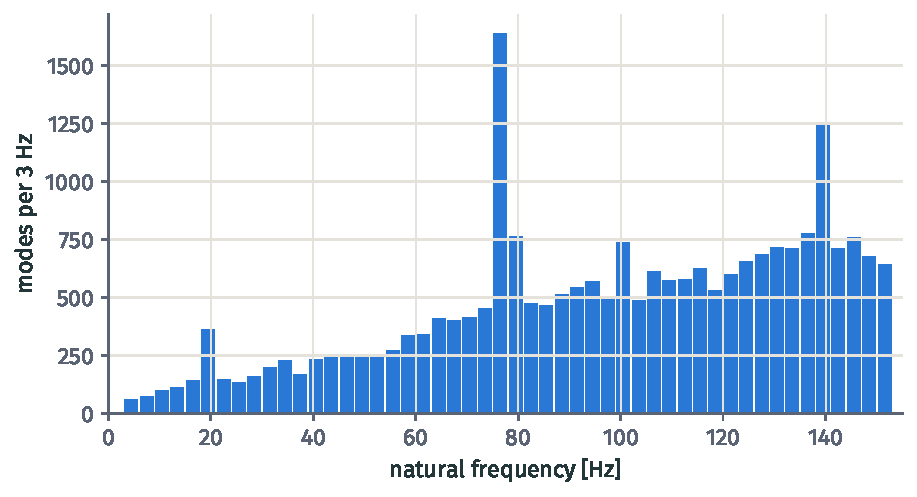
\includegraphics[width=\linewidth]{figures/fem_modes.pdf}

      {\footnotesize Natural frequencies of the M1 fans FEM: 169 modes below \SI{10}{Hz}.}
    \end{column}
  \end{columns}
\end{frame}

%------------------------------------------------------------------------------
\begin{frame}{Servo-mechanisms in the structural simulation}
  The structure is simulated in closed loop with its own controllers, all holding \alert{zero set-points}:
  \vspace{2mm}
  \begin{columns}[T]
    \begin{column}{0.32\textwidth}
      \begin{block}{Mount}
        Azimuth, elevation and GIR drives and encoders (\SI{1}{kHz} controller): reject the wind torque on the mount
      \end{block}
    \end{column}
    \begin{column}{0.32\textwidth}
      \begin{block}{M1}
        6 hardpoints and up to 335 force actuators per segment; the actuators off-load the hardpoint forces (loop sampled at \SI{12.5}{Hz})
      \end{block}
    \end{column}
    \begin{column}{0.32\textwidth}
      \begin{block}{M2}
        Segment positioners (hexapods) and FSM piezo-stack actuators
      \end{block}
    \end{column}
  \end{columns}
  \vspace{4mm}

  \begin{itemize}
    \item Output: the 6 rigid body motions (Tx, Ty, Tz, Rx, Ry, Rz) of the 14 segments, at \SI{1}{kHz}
    \item No optical feedback in stage 1: the residual RBMs are the \alert{open-loop} wavefront disturbance
  \end{itemize}
\end{frame}

%------------------------------------------------------------------------------
\begin{frame}{Optics: from rigid body motions to segment piston}
  \begin{columns}[c]
    \begin{column}{0.55\textwidth}
      \begin{itemize}
        \item \textbf{Linear optical model (LOM)}: sensitivity matrices computed by ray tracing the GMT optics
          \[ p = S_p\,r, \qquad t = S_t\,r \]
          $r$: 84 M1 \& M2 RBMs, $p$: 7 segment pistons, $t$: 14 segment tip-tilts
        \item Segment piston: mean of the wavefront over each segment in the exit pupil
        \item Piston comes from the M1 \& M2 axial motions and, on the off-axis segments S1--S6, also from the segment tilts
      \end{itemize}
    \end{column}
    \begin{column}{0.4\textwidth}
      \begin{alertblock}{Two outputs per case}
        \begin{description}
          \item[open loop] piston of the RBMs from the structural simulation
          \item[FSM] piston after correcting the segment tip-tilt with the M2 fast steering mirrors
        \end{description}
      \end{alertblock}
    \end{column}
  \end{columns}
\end{frame}

%------------------------------------------------------------------------------
\begin{frame}{The FSM tip-tilt loop}
  \begin{columns}[c]
    \begin{column}{0.45\textwidth}
      \begin{itemize}
        \item Sensor: segment tip-tilt from the LOM, averaged over 5 samples (\SI{200}{Hz} frame rate)
        \item Controller: double integrator, gains 0.1376 and 0.0719
        \item Latency: \SI{6}{ms}, plus \SI{1}{ms} to apply the command
        \item Actuator: FSM, \SI{25}{Hz}, $\zeta=0.707$
        \item Correction applied to M2 Rx \& Ry through the inverse of the M2 tilt sensitivity
      \end{itemize}
      \vspace{1mm}
      {\small The FSM does not sense piston: it changes piston only by moving the M2 segments.}
    \end{column}
    \begin{column}{0.53\textwidth}
      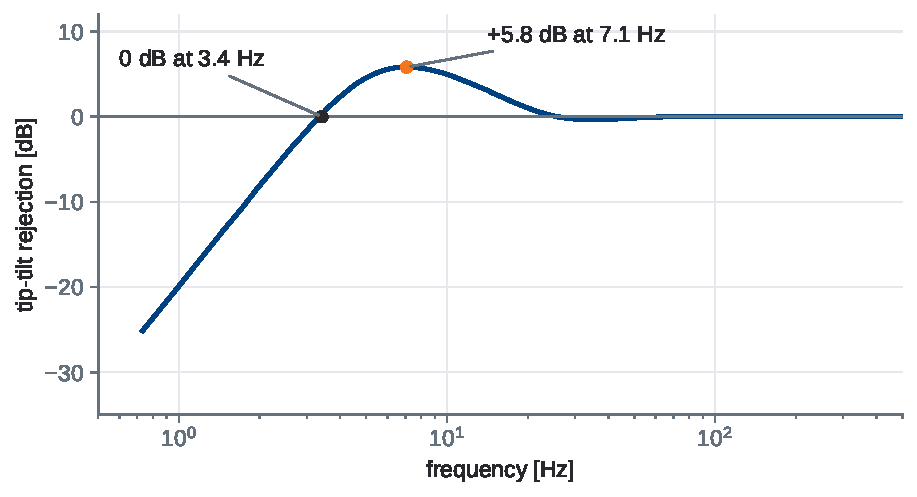
\includegraphics[width=\linewidth]{figures/fsm_rtf.pdf}

      {\footnotesize Rejection transfer function of the loop model, estimated with white noise: \SI{-20}{dB} at \SI{1}{Hz}, transparent above \SI{\sim 25}{Hz}.}
    \end{column}
  \end{columns}
\end{frame}

%------------------------------------------------------------------------------
\begin{frame}{Data pipeline on AWS}
  \centering
  \resizebox{0.97\linewidth}{!}{%
  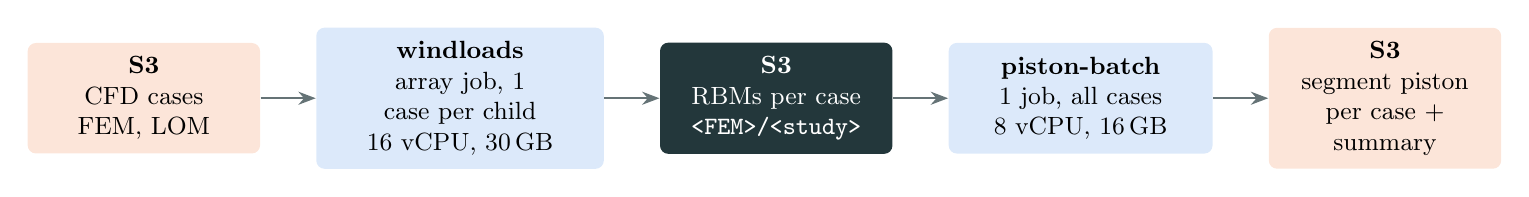
\begin{tikzpicture}[node distance=5mm and 7mm]
    \node[box=softwarm,text width=2.6cm] (s3in) {\textbf{S3}\\CFD cases\\FEM, LOM};
    \node[box=softblue,text width=3.3cm,right=of s3in] (w) {\textbf{windloads}\\array job, 1 case per child\\16 vCPU, \SI{30}{GB}};
    \node[box=ink,text=white,text width=2.6cm,right=of w] (r) {\textbf{S3}\\RBMs per case\\\texttt{<FEM>/<study>}};
    \node[box=softblue,text width=3cm,right=of r] (p) {\textbf{piston-batch}\\1 job, all cases\\8 vCPU, \SI{16}{GB}};
    \node[box=softwarm,text width=2.6cm,right=of p] (s3out) {\textbf{S3}\\segment piston\\per case + summary};
    \draw[flow] (s3in) -- (w);
    \draw[flow] (w) -- (r);
    \draw[flow] (r) -- (p);
    \draw[flow] (p) -- (s3out);
  \end{tikzpicture}}
  \vspace{5mm}

  \begin{columns}[T]
    \begin{column}{0.48\textwidth}
      \begin{itemize}
        \item Containers built from the Rust crates (\texttt{gmt\_dos-actors} framework)
        \item A trade study (FEM, damping) is a new \texttt{<FEM>/<study>} folder: baseline data never overwritten
        \item piston-batch waits for the windloads array job to complete
      \end{itemize}
    \end{column}
    \begin{column}{0.48\textwidth}
      \small
      \begin{tabular}{@{}lr@{}}
        \toprule
        windloads, 1 case alone & \SI{\sim 1}{h}\\
        windloads, 16 cases at a time & \SI{\sim 4.7}{h} median\\
        63 cases, wall clock & \SI{15}{h}\\
        piston-batch, 63 cases & \SI{2}{min}\\
        \bottomrule
      \end{tabular}
    \end{column}
  \end{columns}
\end{frame}

%------------------------------------------------------------------------------
\begin{frame}{Validation}
  \begin{columns}[T]
    \begin{column}{0.5\textwidth}
      \textbf{Stage 1}: rerun of the 2025 baseline (previous FEM, \SI{2}{\%} damping, zen30az000\_OS\_7ms)
      \vspace{1mm}

      \small
      \begin{tabular}{@{}lrrr@{}}
        \toprule
        Piston std [nm] & 2025 & rerun & change\\
        \midrule
        S1--S6 & 578--810 & 578--809 & ${\le}\,0.2\,\%$\\
        S7 & 267.3 & 262.6 & $-1.8\,\%$\\
        \bottomrule
      \end{tabular}

      \vspace{1mm}
      RBM differences: \SI{1.6}{\%} of the RBM std (median), attributed to newer servo-mechanism libraries
    \end{column}
    \begin{column}{0.46\textwidth}
      \textbf{Stage 2}: the FSM loop, ported from the 2025 processing, gives \alert{sample-for-sample identical} RBMs
      \vspace{3mm}

      \textbf{Consequence}: trade studies are compared with reruns made with the same software, so only the changed parameter differs
    \end{column}
  \end{columns}
\end{frame}

%------------------------------------------------------------------------------
\section{Sensitivity to the damping}

\begin{frame}{M1 fans FEM: \SI{2}{\%} against \SI{1}{\%} damping}
  \begin{columns}[c]
    \begin{column}{0.6\textwidth}
      \small
      Open-loop segment piston [nm], zen30az000\_OS\_7ms
      \vspace{1mm}

      \begin{tabular}{@{}lrrrrr@{}}
        \toprule
        & \multicolumn{2}{c}{Total std} & \multicolumn{3}{c}{\SIrange{3}{153}{Hz}}\\
        \cmidrule(lr){2-3}\cmidrule(l){4-6}
        Segment & \SI{2}{\%} & \SI{1}{\%} & \SI{2}{\%} & \SI{1}{\%} & change\\
        \midrule
        S1 & 774.1 & 775.2 & 68.3 & 78.0 & $+14\,\%$\\
        S2 & 608.1 & 610.2 & 60.2 & 72.9 & $+21\,\%$\\
        S3 & 677.7 & 679.6 & 70.4 & 79.4 & $+13\,\%$\\
        S4 & 811.5 & 813.1 & 51.8 & 65.5 & $+26\,\%$\\
        S5 & 726.1 & 727.7 & 73.3 & 83.1 & $+13\,\%$\\
        S6 & 578.4 & 580.2 & 81.4 & 90.6 & $+11\,\%$\\
        S7 & 262.4 & 265.4 & 38.0 & 48.0 & $+26\,\%$\\
        \bottomrule
      \end{tabular}
    \end{column}
    \begin{column}{0.36\textwidth}
      \begin{itemize}
        \item Total std: $+0.2$ to $+1.1\,\%$
        \item Below \SI{1}{Hz}: unchanged (within \SI{0.4}{nm})
        \item Resonant band, \SIrange{3}{153}{Hz}: $+11$ to $+26\,\%$
        \item FSM values within \SI{0.5}{\%} of open loop
      \end{itemize}
      \vspace{1mm}
      {\small The damping only acts on the structural resonances; most of the piston is quasi-static.}
    \end{column}
  \end{columns}
\end{frame}

%------------------------------------------------------------------------------
\begin{frame}{Damping: the resonances grow above \SI{3}{Hz}}
  \centering
  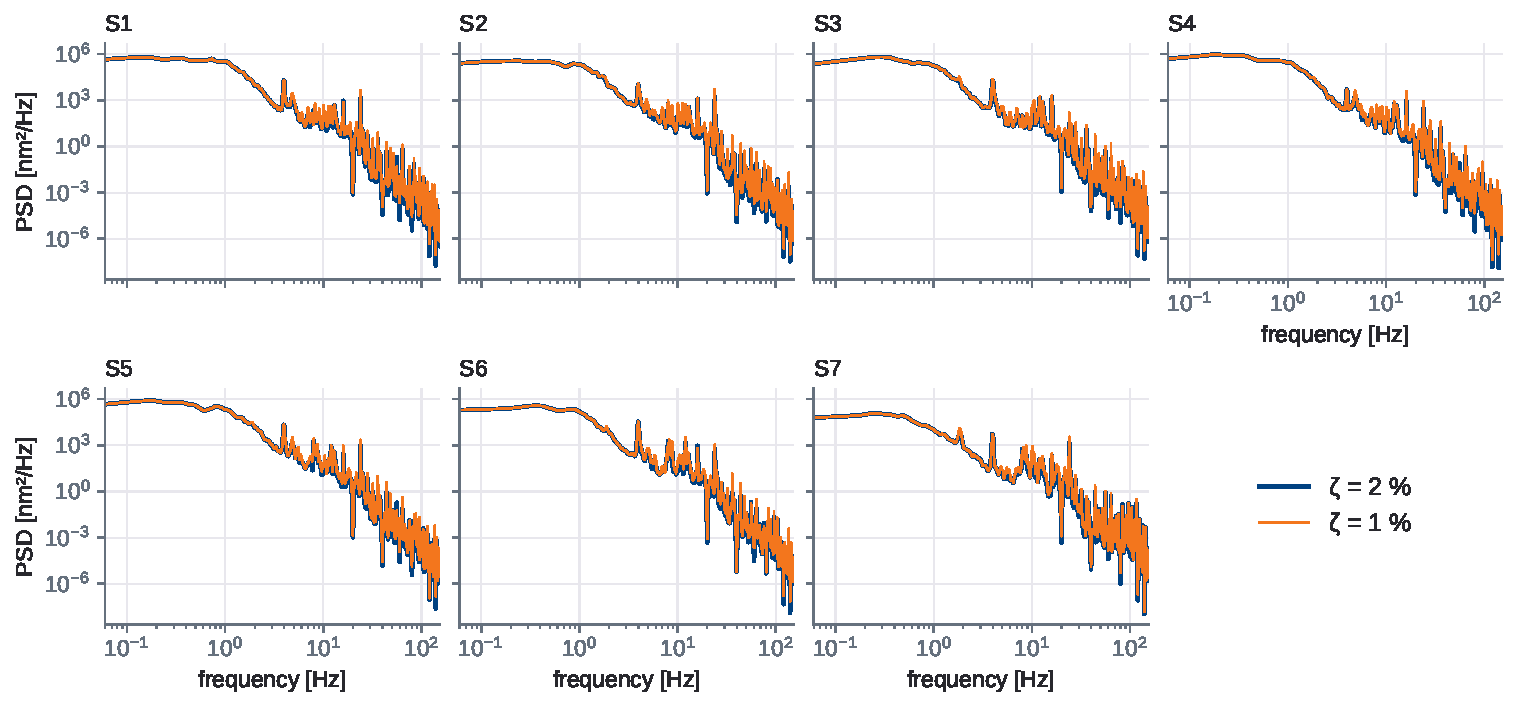
\includegraphics[width=0.92\linewidth]{figures/damping_psd.pdf}

  {\small Open-loop segment piston PSDs, M1 fans FEM, zen30az000\_OS\_7ms, \SIrange{0.06}{153}{Hz}}
\end{frame}

%------------------------------------------------------------------------------
\begin{frame}{Damping: the curves separate above \SI{3}{Hz}}
  \centering
  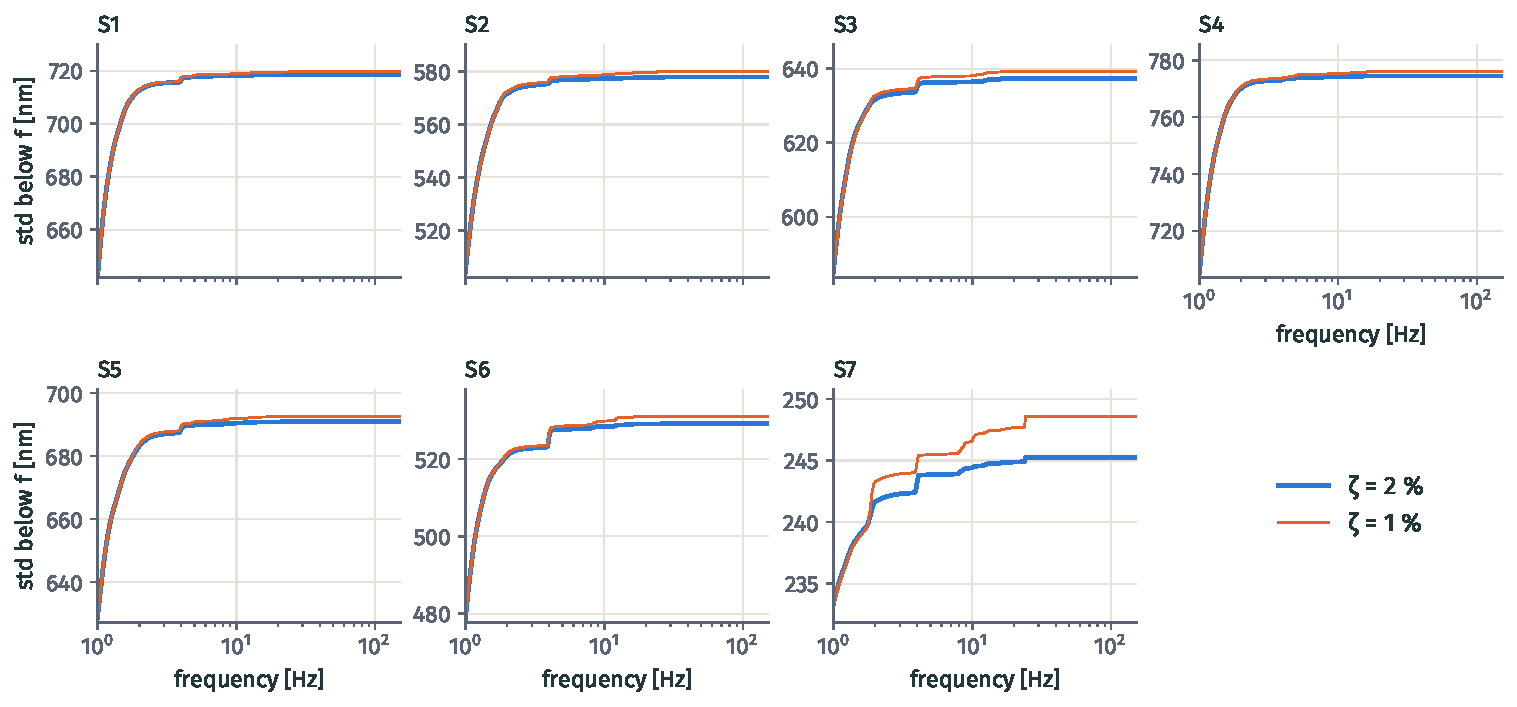
\includegraphics[width=0.86\linewidth]{figures/damping_cumstd.pdf}

  {\small $\sigma(f)=\sqrt{\int_0^f \mathrm{PSD}}$, \SIrange{1}{153}{Hz}, y axes zoomed: the curves overlap up to \SI{\sim 3}{Hz}, then each mode adds a step, larger at \SI{1}{\%}: $+$\SIrange{1}{2}{nm} on S1--S6, $+$\SI{3}{nm} on S7}
\end{frame}

%------------------------------------------------------------------------------
\section{Segment piston over the 63 CFD cases}

\begin{frame}{63 cases, M1 fans FEM, \SI{1}{\%} damping}
  \centering
  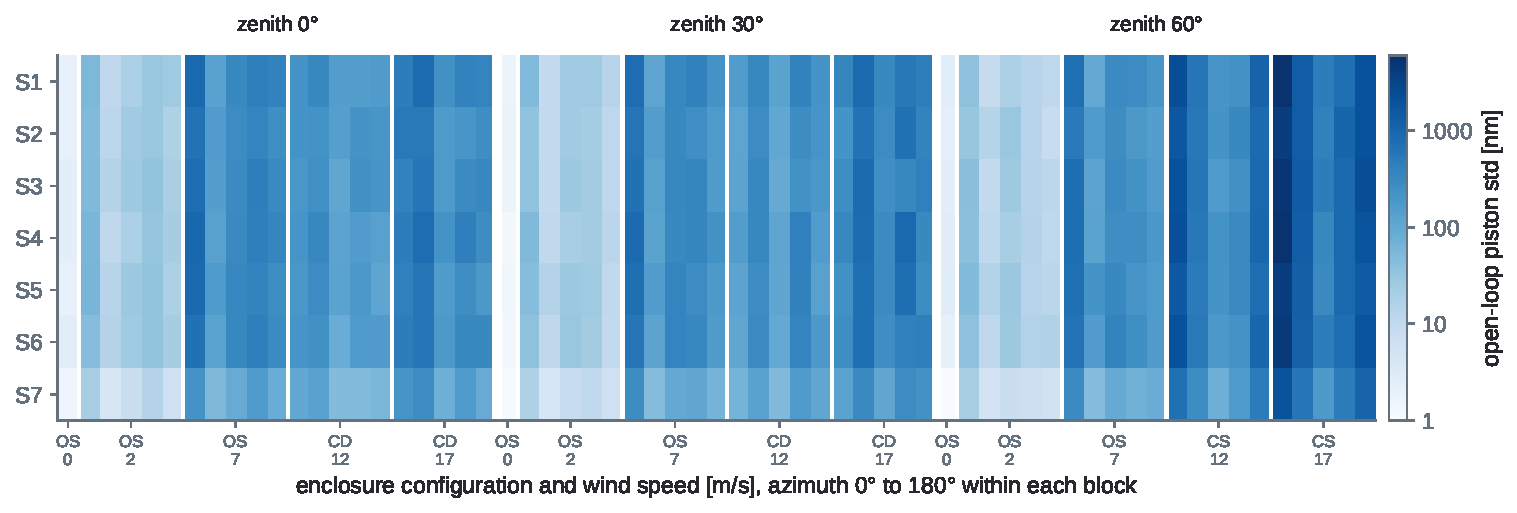
\includegraphics[width=\linewidth]{figures/cases_heatmap.pdf}

  {\small Open-loop segment piston std per segment and case (log scale). The \SI{0}{m/s} cases give \SI{\sim 2}{nm}; the worst case is zenith \ang{60}, closed vents, \SI{17}{m/s}.}
\end{frame}

%------------------------------------------------------------------------------
\begin{frame}{Piston grows with wind speed, most at zenith \ang{60}}
  \centering
  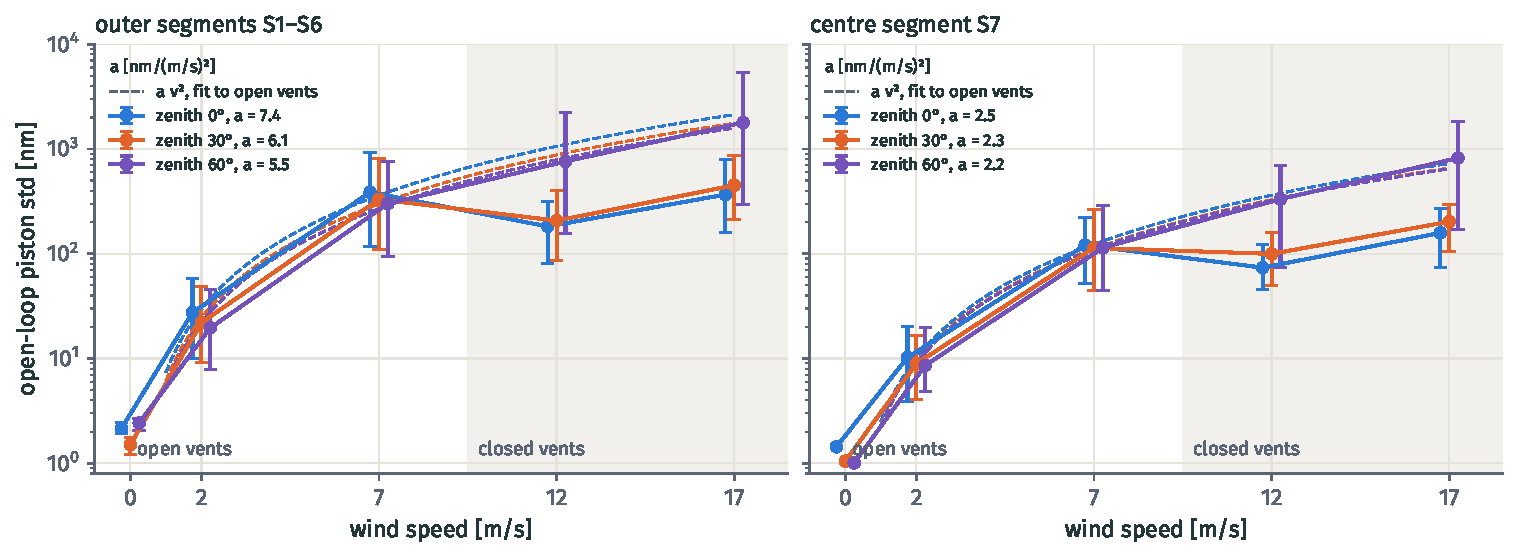
\includegraphics[width=0.86\linewidth]{figures/std_vs_wind.pdf}

  {\small Mean over the 5 azimuths (and over S1--S6, left); bars span the minimum and maximum over azimuths and segments. With closed vents and the wind screen deployed (CD), \SI{12}{m/s} gives less piston than \SI{7}{m/s} with open vents; at zenith \ang{60} the screen is stowed (CS) and the piston keeps growing.}
\end{frame}

%------------------------------------------------------------------------------
\begin{frame}{Segment piston statistics}
  \small
  Open-loop segment piston std [nm], mean and maximum over the 5 azimuths
  \vspace{1mm}

  \centering
  \begin{tabular}{@{}llrrrr@{}}
    \toprule
    & & \multicolumn{2}{c}{S1--S6} & \multicolumn{2}{c}{S7}\\
    \cmidrule(lr){3-4}\cmidrule(l){5-6}
    Zenith & Enclosure, wind & mean & max & mean & max\\
    \midrule
    \ang{0}  & OS 2 / \SI{7}{m/s}  & 28 / 386 & 58 / 934 & 10 / 121 & 20 / 221\\
             & CD 12 / \SI{17}{m/s} & 182 / 367 & 318 / 787 & 74 / 158 & 122 / 271\\
    \ang{30} & OS 2 / \SI{7}{m/s}  & 22 / 331 & 49 / 813 & 9 / 114 & 17 / 265\\
             & CD 12 / \SI{17}{m/s} & 207 / 451 & 403 / 871 & 100 / 202 & 159 / 293\\
    \ang{60} & OS 2 / \SI{7}{m/s}  & 20 / 301 & 46 / 754 & 9 / 114 & 20 / 291\\
             & CS 12 / \SI{17}{m/s} & 760 / \alert{1785} & 2218 / \alert{5415} & 332 / 820 & 696 / 1833\\
    \bottomrule
  \end{tabular}
  \vspace{3mm}

  \raggedright
  Median over all cases and outer segments: \SI{211}{nm}. Worst case zen60az000\_CS\_17ms: \SIrange{3.6}{5.4}{\micro m} on S1--S6. S7 is 2 to 3 times lower than the outer segments. At \SI{0}{m/s}: \SI{\le 3}{nm}.
\end{frame}

%------------------------------------------------------------------------------
\begin{frame}{Temporal spectrum: the piston is slow}
  \centering
  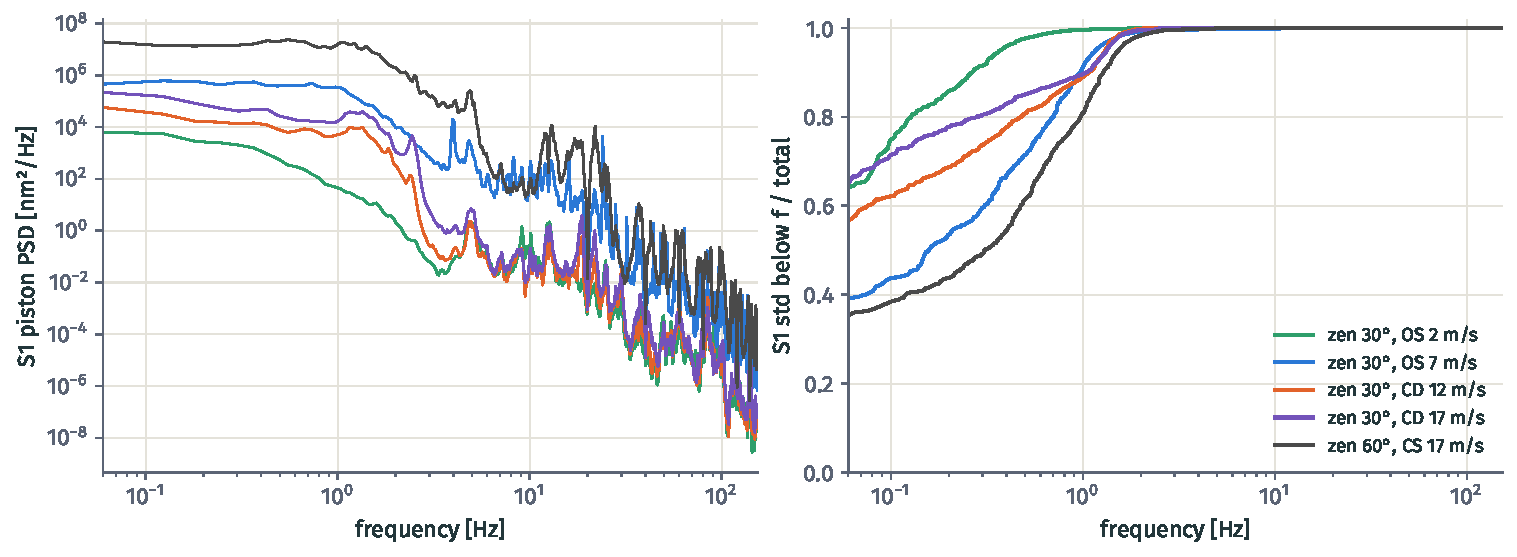
\includegraphics[width=0.88\linewidth]{figures/cases_psd.pdf}

  {\small S1 open-loop piston at azimuth \ang{0}: 78 to 99\,\% of the std is below \SI{1}{Hz} and more than 99\,\% below \SI{3}{Hz}, for all wind speeds. Above \SI{3}{Hz} the spectrum is set by the structural modes (\SIrange{4}{25}{Hz}).}
\end{frame}

%------------------------------------------------------------------------------
\begin{frame}{The FSM does not reduce the piston}
  \begin{columns}[c]
    \begin{column}{0.55\textwidth}
      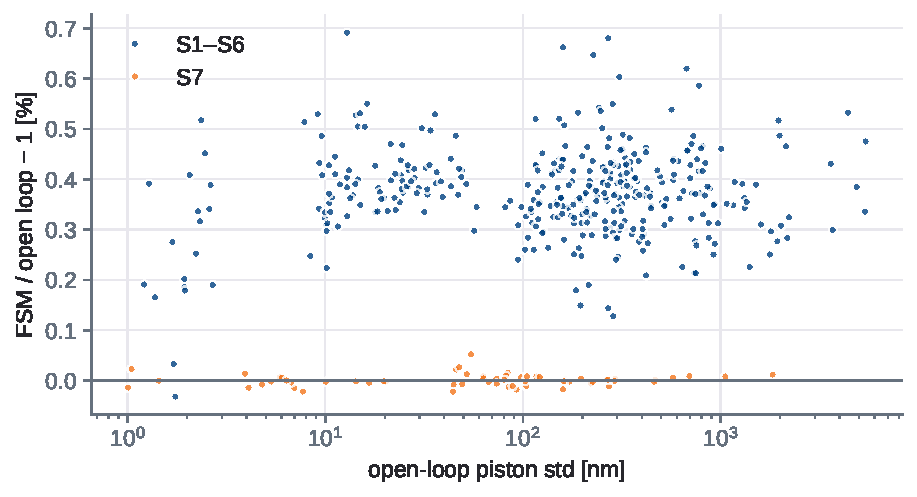
\includegraphics[width=\linewidth]{figures/fsm_ratio.pdf}
    \end{column}
    \begin{column}{0.39\textwidth}
      \begin{itemize}
        \item S1--S6: the FSM \alert{adds} \SI{0.37}{\%} piston std on average (\SIrange{-0.03}{0.7}{\%})
        \item S7: unchanged (within \SI{0.05}{\%})
        \item The M2 tilts that correct the segment tip-tilt couple into piston on the off-axis segments
        \item Piston is left to the phasing control: with ${>}\,99\,\%$ of the std below \SI{3}{Hz}, a rejection bandwidth of a few Hz covers most of it
      \end{itemize}
    \end{column}
  \end{columns}
\end{frame}

%------------------------------------------------------------------------------
\begin{frame}{Summary}
  \begin{columns}[T]
    \begin{column}{0.48\textwidth}
      \begin{block}{Pipeline}
        \begin{itemize}
          \item CFD loads $\rightarrow$ FEM + servo-mechanisms $\rightarrow$ RBMs $\rightarrow$ LOM piston, open loop and with the FSM
          \item Reproducible trade studies on AWS Batch, validated against the 2025 baseline
        \end{itemize}
      \end{block}
      \begin{block}{Damping (M1 fans FEM)}
        \begin{itemize}
          \item $\zeta$: \SI{2}{\%} $\rightarrow$ \SI{1}{\%}: total piston $+0.2$ to $+1.1\,\%$, resonant band ($>$\SI{3}{Hz}) $+11$ to $+26\,\%$
        \end{itemize}
      \end{block}
    \end{column}
    \begin{column}{0.48\textwidth}
      \begin{block}{63 CFD cases (\SI{1}{\%} damping)}
        \begin{itemize}
          \item Outer segments: \SI{20}{nm} to \SI{1.8}{\micro m} std (configuration means, \SI{0}{m/s} excluded), median \SI{211}{nm}
          \item Worst: zenith \ang{60}, closed vents, \SI{17}{m/s}: up to \SI{5.4}{\micro m}
          \item $>$\,99\,\% of the piston std below \SI{3}{Hz}
          \item The FSM leaves the piston unchanged ($+0.4\,\%$)
        \end{itemize}
      \end{block}
      {\small Damping sensitivity from one CFD case only; the 63 cases at \SI{2}{\%} would complete the trade.}
    \end{column}
  \end{columns}
\end{frame}

\end{document}
